\documentclass[11pt,a4paper]{article}
\usepackage[ngerman]{babel}
\usepackage{graphicx}
\usepackage{float}
\usepackage[textfont=it, width= 0.75\textwidth, textformat=period, labelformat=empty, justification=RaggedRight, singlelinecheck=false]{caption}
\usepackage[labelformat=empty]{subcaption}
\usepackage{wrapfig}
\usepackage{wallpaper}
\usepackage{booktabs}
\usepackage{amsmath}
\usepackage{esvect}
\usepackage{url}
\usepackage{lmodern}
\usepackage[colorlinks=true,linkcolor=black,urlcolor=cyan,citecolor=black]{hyperref}
\usepackage[left=2.5cm,right=2.5cm,top=2cm,bottom=2cm]{geometry}

%Konfiguration von Absätzen
\setlength{\parindent}{0pt}
\setlength{\parskip}{4pt}

\addtolength{\wpXoffset}{-6,3cm}

\begin{document}
\thispagestyle{empty}

%\ThisCenterWallPaper{0.9}{Bilder/FTV-Darstellung.png} %Hintergrundbild von FTV

{\scshape\large\centering Gymnasium Eversten Oldenburg \\}
\vspace{-10pt}
\noindent\rule{\textwidth}{0.5pt} %Horizontale Linie
\vspace{5pt}
{\large\bfseries\centering Aerodynamik von Modellraketen: Luftwiderstand und Flugstabilität \\}
\vspace{-6pt}
{\centering \url{https://github.com/FTVLab/Aerodynamik-von-Modellraketen} \\}
\vspace{-2pt}
{\centering\sffamily\scshape Jeremias Beth und Benjamin Lips \\}

\vspace{-5pt}
\paragraph{Zielsetzung}
In dieser Arbeit wird der Einfluss der Raketenspitze auf den Flug einer Modellrakete untersucht. Diese Untersuchung findet anhand der selbst gebauten Rakete FTV statt, wobei Luftwiderstand und Flugstabilität untersucht wurden. Es wurden fünf Formen von Raketenspitzen betrachtet.

\vspace{-10pt}
\paragraph{Luftwiderstand}
Die Untersuchung des Luftwiderstandes hat das Ziel, von den Spitzen die mit der grö"sten Flughöhe zu ermitteln. Dafür wird im Windkanal der Widerstandsbeiwert von FTV mit jeder der Spitzen bestimmt. Anschlie"send wird ein möglichst simples Modell entwickelt, mit dem der Flug wird. 

\begin{figure}[H]
	\begin{subfigure}[l]{0.49\textwidth}
		\centering
		\includegraphics[width=\textwidth]{Bilder/Flugsimulation-C6-5.png}
		\caption{Flugsimulation von FTV mit \textsf{C6-5}-Treibsatz}
		\label{sfig-Flugsimulation}
	\end{subfigure}
	\begin{subfigure}[r]{0.49\textwidth}
		\centering
		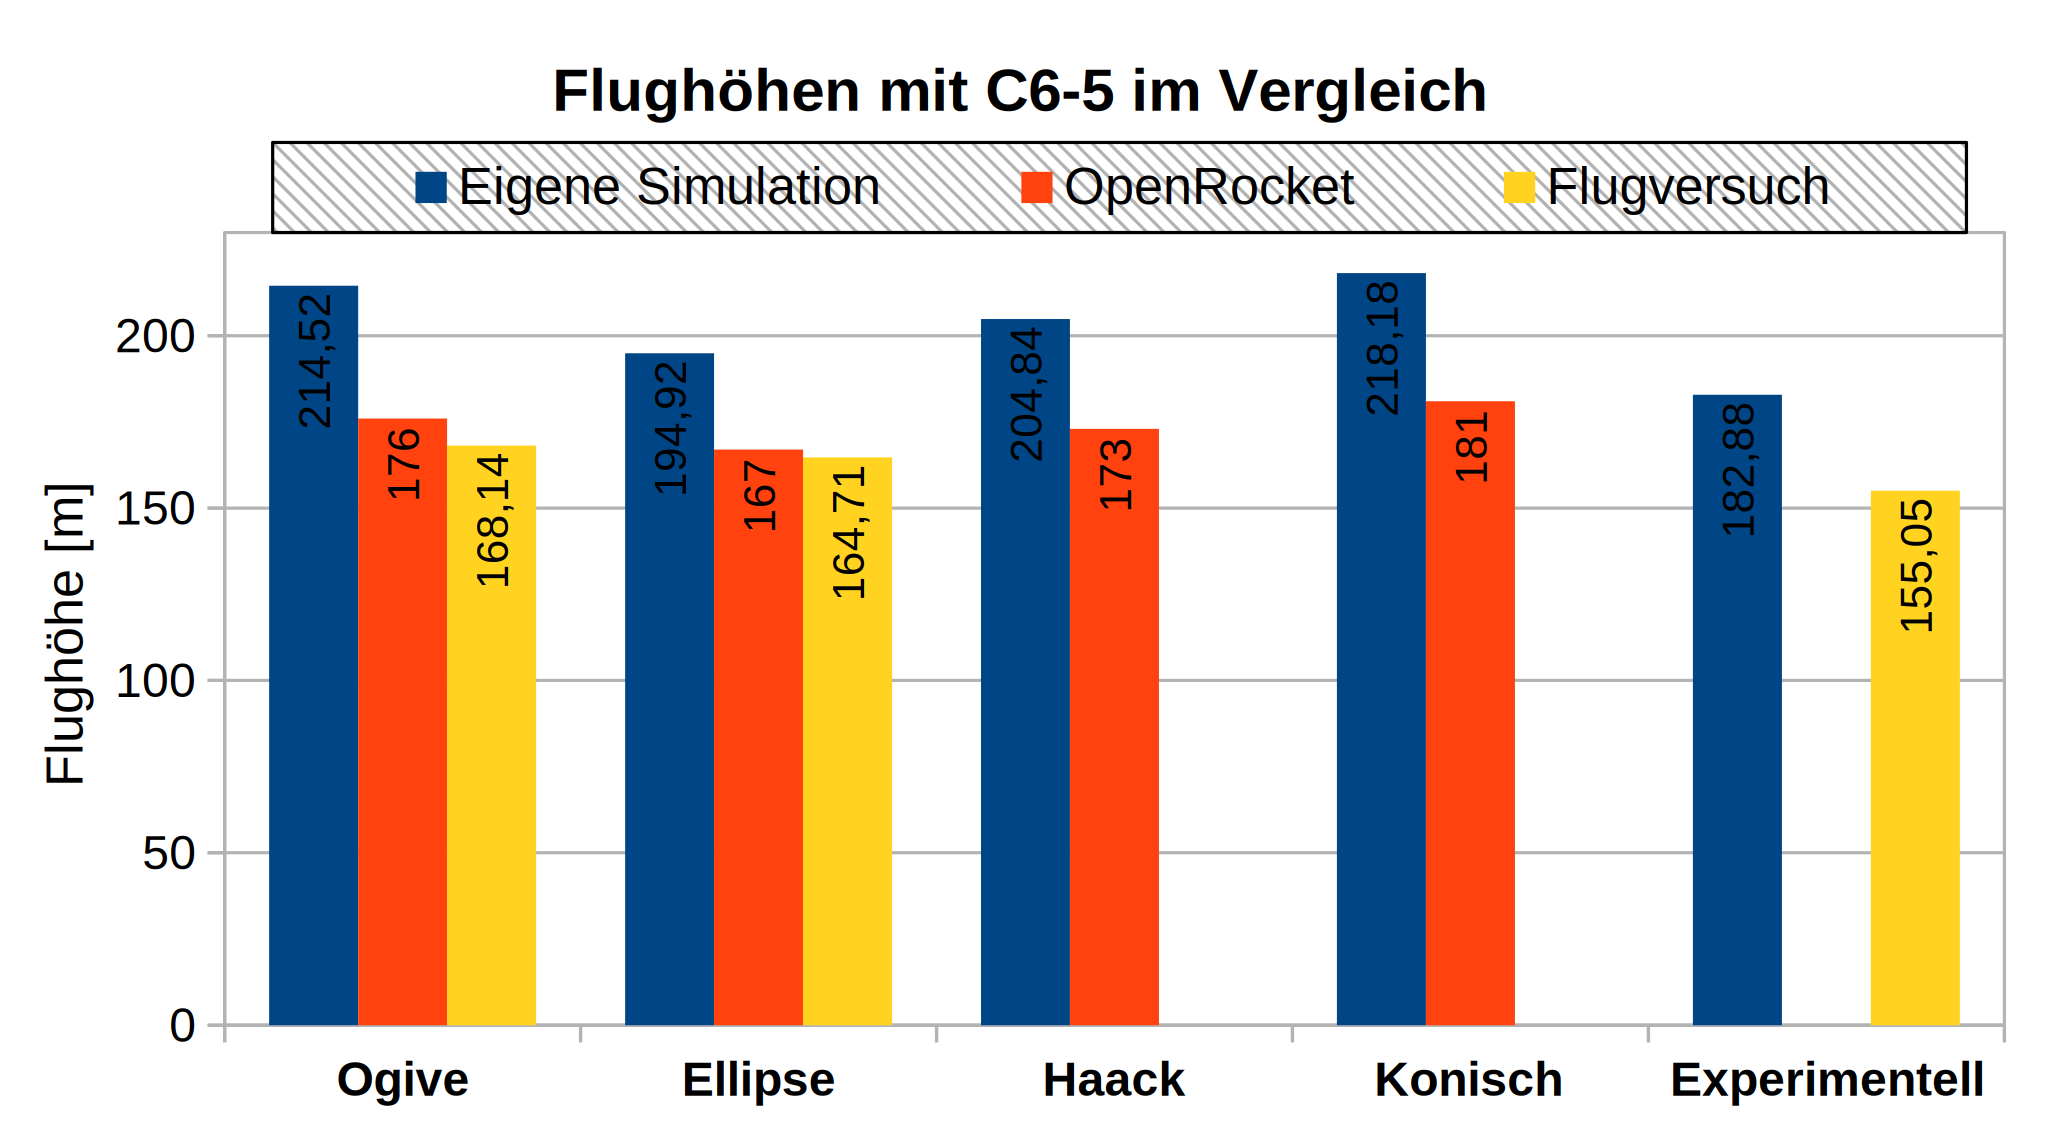
\includegraphics[width=\textwidth]{Bilder/Flughöhen-Vergleich.png}
		\caption{Vergleich der simulierten Flughöhe}
		\label{sfig-Simulierte-Flughöhe}
	\end{subfigure}
\end{figure}

\vspace{-10pt}
\begin{wrapfigure}{r}{0.3\textwidth}
	\vspace{-11pt}
	\centering
	\includegraphics[width=0.3\textwidth]{Bilder/Flugversuch-Start.jpg}
	\caption{FTV während des Starts}
\end{wrapfigure}

Der Versuch ergab, dass die Ogive als Spitzenform im Unterschallbereich den geringsten Luftwiderstand aufweist. In der Simulation zeigte sich jedoch, dass die leichte konische Spitze der Ogive im niedrigen Unterschallbereich eine grö"sere Flughöhe aufweist. Für grö"sere Geschwindigkeiten nimmt der aerodynamische Einfluss zu, sodass die Ogive höher fliegt. Die Hypothese, dass ein knickfreier Übergang zwischen Körperrohr und Spitze den Luftwiderstand verringert, wurde bestätigt.

\vspace{-10pt}
\paragraph{Flugstabilität}
Die Untersuchung der Flugstabilität fand zunächst theoretisch statt, wobei ein Verfahren zur Berechnung des Druckpunktes eingesetzt wurde.
Die theoretische Untersuchung ergab, dass FTV mit allen Spitzen ausreichende Flugstabilität aufweist. Diese Ergebnisse konnten durch den Versuch im Windkanal bestätigt werden, wobei zusätzlich festgestellt wurde, dass sich die Rakete quer zum Wind stabil ausrichten kann. Das ist jedoch im Flug sehr unwahrscheinlich.

Flugversuche zeigten ebenfalls stabiles Flugverhalten. Die Ausrichtung quer zum Wind trat beim herabfallen der Rakete auf. Dadurch wurde FTV trotz Fehlfunktion des Bergungssystems im Fall gebremst und nicht beschädigt.

Im Vergleich der Spitzen lässt sich keine als optimal feststellen. Welche Spitze für eine konkrete Rakete in Bezug auf die Flugstabilität am besten ist, hängt davon ab, ob eine zu gro"se oder kleine Kaliberzahl vorliegt.



\end{document}